\documentclass[12pt, openany]{article}
\usepackage[utf8]{inputenc}
\usepackage[T1]{fontenc}
\usepackage[a4paper,left=2.5cm,right=2.5cm,top=3cm,bottom=3cm]{geometry}
\usepackage[frenchb]{babel}
\usepackage{libertine}
\usepackage[pdftex]{graphicx}
\usepackage{graphicx}
\usepackage{setspace}
\graphicspath{ {./images/} }
\setlength{\parindent}{1cm}
\setlength{\parskip}{2ex plus 5ex minus 0.2ex}
\newcommand{\hsp}{\hspace{20pt}}
\newcommand{\HRule}{\rule{\linewidth}{0.5mm}}
\setlength\itemsep{1cm}

\begin{document}

\begin{titlepage}
  \begin{sffamily}
  \begin{center}
    
    \textsc{\LARGE École Polytechnique} \\[0.5cm]

    \textsc{\Large PSC}\\[4cm]

    % Title
    \HRule \\[0.4cm]
    { \huge \bfseries Proposition Détaillée\\[0.4cm] Surveillance de zone par réseau de drones \\[0.4cm] }

    \HRule \\[6cm]

    % Author and supervisor
    \begin{minipage}{0.4\textwidth}
      \begin{flushleft} \large
        \textsc{Paul Mortamet\\
        Thibault Vignon\\
        Louis Proffit\\
        Louis Stefanuto\\
        X2019\\}
      \end{flushleft}
    \end{minipage}
    \begin{minipage}{0.4\textwidth}
      \begin{flushright} \large
      \textsc{
        \emph{Tuteur :} \\
        M. Vincent Jeauneau\\
        \medbreak \\
        \emph{Coordinateur : } \\
        M. Emmanuel Haucourt \\}
      \end{flushright}
    \end{minipage} \\[1cm]
    
    \textsc{\large 25 Septembre 2020 }
    
    
  \end{center}
  \end{sffamily}
\end{titlepage}

\newpage
\section{Enjeux et motivation du travail, objectif final}
\vspace{1cm}

Le 9 juillet 2016, la police de Dallas tue un tireur embusqué à l’aide d’un drone explosif. En janvier 2019, une attaque de drones tue six officiers de l’armée loyaliste Yéménite. Le 14 septembre de la même année, des drones armés ravagent un site pétrolier en Arabie Saoudite et détruisent près de la moitié des capacités de production de la société pétrolière, soit 5 \% des capacités de production mondiales de pétrole brut. Ces quelques exemples parmi tant d’autres illustrent l’émergence des drones dans la façon de faire la guerre ou d’attaquer une force ennemie.

Mais l’utilisation des drones de combat par les forces armées majeures n’est pas un phénomène nouveau et remonte même à la Seconde Guerre Mondiale avec les missiles de croisière. Néanmoins, la démocratisation des drones miniatures, voire domestiques, associée à la progression exponentielle des technologies d’automatisation et d’intelligence artificielle ont rendus les frappes à distance pratiques beaucoup plus accessibles. Parfaitement adaptés pour les actes de terrorismes, d’espionnage ou pour les attaques officieuses de gouvernements malveillants, les drones miniatures menacent dorénavant les sites stratégiques militaires ou civils autant que les concerts publics, les manifestations urbaines, les évènements sportifs ou les meetings politiques. 

Les technologies permettant d’éliminer chirurgicalement une classe de la population selon le sexe, l’âge ou les opinions exposées sur internet nous paraissent fantaisistes. Le seront-elles longtemps ? De nos jours, aucun système de défense anti-aérien déployé n’a été pensé pour contrer une attaque de drones de taille réduite ou artisanaux. Trop petits, ces robots ne sont pas détectés par les moyens de surveillance militaires actuels et le nombre d’assaillant sature rapidement les moyens de neutralisation. Évoluant proche du sol, ces drones nécessitent un traitement à part : utiliser un nuage de drones pour défendre une zone d’attaque potentielle est la solution qui nous a paru la plus intéressante. Cette technique permet d’utiliser la mobilité, la maniabilité, la modularité des drones contre eux-mêmes tout en essayant d’apporter une organisation tactique conséquente, qui est le point faible des attaques de drones terroristes.

Les systèmes de défense anti-drones miniatures nous interpellent car ils semblent être une pierre angulaire de la défense de demain. En tant qu’élèves-officiers des armées françaises, mettre en œuvre nos compétences académiques pour apporter une partie de solution à cet enjeu majeur pour les armées nous semble crucial. Ce projet nous permettra de développer des compétences en informatique, domaine incontournable du métier d’ingénieur de demain. 

Nous sommes conscients de l’ampleur du problème c’est pourquoi nous avons choisi de nous focaliser sur la solution des nuages de drones, bien que de nombreuses autres pistes sont exploitables et même exploitées actuellement. Dans la solution potentielle qu’est le nuage de drones, nous souhaitons nous concentrer sur l'implémentation des algorithmes, et pas la mise en pratique des solutions qui nécessite des moyens financiers importants, et de fortes contraintes en matière de sécurité.

Notre PSC se place dans la continuité du PSC d'un groupe de la promotion X2018, qui avait étudié le même sujet. Nous poursuivrons leur recherches en nous basant sur ce qu'ils ont produit et utilisé. Ils ont notamment orienté leur recherches vers l'algorithme A*, algorithme de parcours de graphes, qui leur permet de chercher un chemin entre deux points en évitant les obstacles, en 2D. Nous implémenterons nos premiers algorithmes sur cette base, avant d'éventuellement l'améliorer (c.f algorithme RHTA, voir plus loin). Le groupe précédent avait également créé une interface graphique (Python) pour visualiser le comportement de leur algorithmes. Nous ferons de même (sur Java) pour la partie 2D. Nous envisageons également d'utiliser le logiciel de conception de jeux vidéo et moteur graphique Unity\texttrademark, dont la prise en main est relativement accessible, pour faire de même en 3D.

L'objectif final de notre PSC est de produire un ou des algorithmes qui orientent un groupe de drones pour la surveillance d'une zone, en garantissant à chaque instant et quel que soit le contexte, que ceux-ci sont en mesure de repérer et d'intercepter une menace. Ces algorithmes s'accompagneront de solutions graphiques pour visualiser le fonctionnement de ces algorithmes.


\newpage
\section{Revue et analyse de l’état de l’art / des approches concurrentes ou alternatives}
\vspace{1cm}

La défense contre des drones malveillants est un domaine où il est difficile de dresser un état de l’art précis, car c’est un sujet qui porte des enjeux militaires conséquents et qui sera probablement l’un des points-clés de la ‘guerre de demain’. En raison de leur caractère sensible, les avancées pratiques dans ce domaine font l’objet d’une communication très limitée et les méthodes utilisées ne sont jamais rendues publiques. De plus, la majorité des systèmes actuels de défense contre des attaques de drones emploient des moyens statiques plutôt qu’un réseau de drones défensif \cite{1}  .

Cependant, en ce qui concerne les fondements théoriques possibles d’un tel système basé sur la coopération d’un essaim de drones de surveillance, la littérature scientifique apporte un panel relativement vaste de réponses. Cela passe notamment par les recherches dans le champ de l’intelligence d’essaim (‘swarm intelligence’). Ce concept, très en vogue au début des années 2000, consiste à chercher à appliquer à un réseau de drones, ou à un système robotisé équivalent, le principe de fonctionnement d’une colonie de fourmis. Les algorithmes d’intelligence d’essaim permettent de faire coopérer un réseau de drones en réduisant au strict minimum la quantité de communication nécessaire. Cette approche a été employée pour résoudre des problèmes tels que la recherche d’intrus dans une zone prédéfinie \cite{2}.

En augmentant l’échange d’informations entre drones et en introduisant un système centralisé d’allocation des tâches entre drones, on peut obtenir des solutions bien plus efficaces. C’est notamment l’objectif de l’algorithme RHTA (Receding Horizon Task Assignment)\cite{3}  , qui utilise une approche heuristique pour arriver à une allocation des tâches proche de l’optimalité tout en ayant un temps de calcul largement inférieur à celui nécessaire pour déterminer la solution exacte. Puisque cet algorithme et d’autres du même type n’ont pas été conçus avec comme objectif la surveillance aérienne, ils ne sont pas tels quels adaptés au système que nous cherchons à concevoir ; cependant, nous pourrons largement nous inspirer de leur approche dans nos recherches.

En se basant sur cet algorithme, Bethke \cite{4}  a proposé un schéma complet d’un réseau coopératif de drones de recherche, comprenant la détection et le suivi de cibles ainsi que la gestion de l’autonomie restante des drones. L’architecture envisagée pour le système de commande de ce réseau est présentée dans le schéma Fig~\ref{fig1} p.~\pageref{fig1}.

En ce qui concerne l’interception, plusieurs techniques de degrés de complexité variés ont été proposées. Bethke \cite{4} montre comment l’estimation des positions successives de la cible permet de gagner en rapidité d’interception par rapport à une approche naïve. Plus récemment, une approche consistant à encercler le drone intrus par un cluster de drones intercepteurs pour l’escorter en dehors de la zone à défendre a été proposée \cite{5} . Les schémas ci-dessous illustrent les étapes de cette méthode d’interception. Même si nous ne retiendrons pas forcément cette solution, elle donne une idée de la diversité de techniques possibles pour intercepter un drone malveillant.
\clearpage
\begin{figure}[!h]
    \vspace{1cm}\\
    \centering
    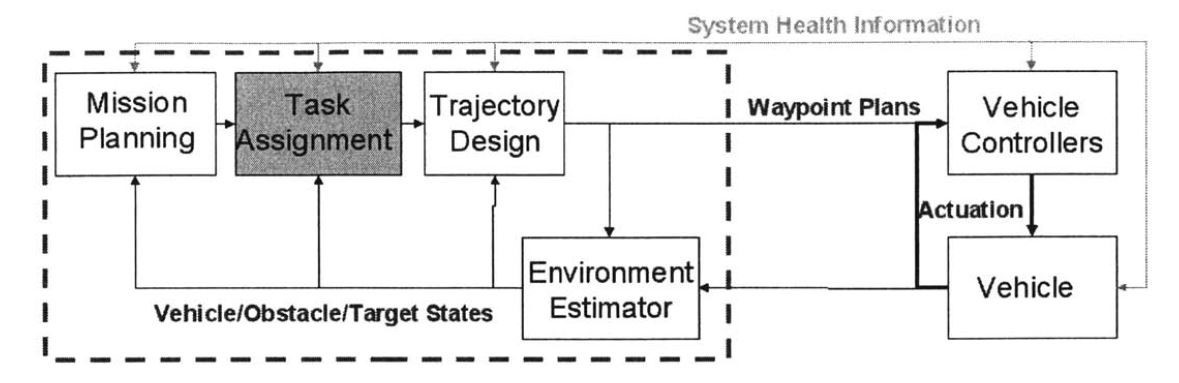
\includegraphics[scale=0.7]{Schéma réseau de drones état de l'art proposition détaillée}
    \caption{Schéma d'un réseau coopératif de drones de recherche}
    \label{fig1}
    \vspace{1cm}\\
\end{figure}

\begin{figure}[!h]
    \vspace{1cm}\\
    \centering
    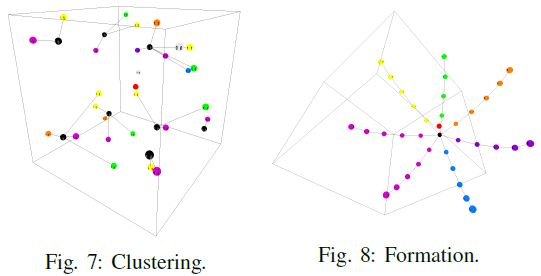
\includegraphics[scale = 1]{interception bulle 1.JPG}
    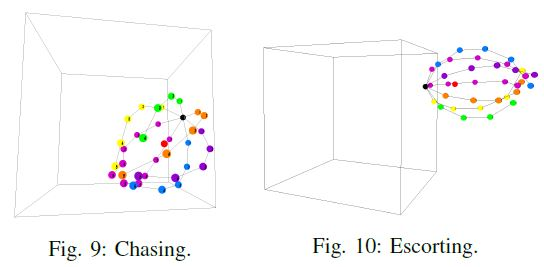
\includegraphics[scale = 1]{interception bulle 2.JPG}
    \caption{Traitement par un réseau de drones d'un intrus en 4 étapes}
    \vspace{1cm}\\
\end{figure}


\newpage
\section{Objectifs intermédiaires et échéancier}
\vspace{1cm}

Voici un descriptif des objectifs intermédiaires, et l'ordre chronologique dans lequel ceux-ci vont s'enchainer. L'objectif final est d'atteindre le point 6, mais les points 7 et 8 proposent des avancées intéressantes au cas où nous atteignons nos objectifs plus tôt que prévu.

\begin{enumerate}
\setlength\itemsep{0.7cm}

\item 
\textbf{Reprise du dossier de l'année précédente}

Déterminer les écueils du groupe antérieur, étudier les partis pris, les solutions mises en œuvre et leurs limites. Cette phase préliminaire sera considérée comme achevée une fois les solutions techniques pour le T1 décidées et l'état de l'art sur le sujet étayé. La proposition détaillée achève cette phase.

\item
\textbf{Solution de tracé de parcours optimal A* et représentation graphique 2D}

Cet algorithme doit permettre de :
\begin{itemize}
    \setlength\itemsep{0.1cm}
    \item Placer des murs sur la grille N×N à l’initialisation dans un 1er temps puis à la souris dans un 2nd.
    \item De placer des points de passage dans un ordre défini dans un 1er temps puis à la souris dans un 2nd.
    \item De calculer, en cas d’ajout d’un point ou d’un obstacle, le nouveau parcours à suivre.
\end{itemize}

\item
\textbf{Amélioration de l'algorithme précédent et répartition des drones sur le parcours}

Ce nouvel algorithme doit permettre de :
\begin{itemize}
    \setlength\itemsep{0.1cm}
    \item Rajouter un drone en cliquant quelque part sur le chemin.
    \item Adapter la vitesse des autres drones pour qu’ils se répartissent uniformément.
    \item Retirer un drone à tout instant et s’adapter de la même façon que pour l’ajout.
    \item Gérer la question du drone qui s’est écarté du chemin, comment revenir «dans la ronde»?
\end{itemize}
	

\item
\textbf{Perfectionnement de l'algorithme}

Avec pour objectif la modularité, on perfectionne l'algorithme en ajoutant un maximum de fonctionnalités :
\begin{itemize}
    \setlength\itemsep{0.1cm}
    \item Découper la zone en fonction d'un critère de "priorité", dont l'algorithme se sert pour privilégier la surveillance des zones les plus importantes.
    \item Rajouter/enlever une zone, modifier son niveau d’importance.
    \item Adapter un algorithme RTHA au problème (gain de performance), qui résout dynamiquement le problème.
\end{itemize}

\item
\textbf{Implémenter en 3D l'algorithme}

Considérer les zones de priorité comme des volumes. Nécessite d'intégrer une représentation par interface graphique 3D (Unity). 

\item
\textbf{Expérimentation}
Test des différents algorithmes produits, comparaison des performances et de la modularité

\item
\textbf{Interception}
\begin{itemize}
    \setlength\itemsep{0.1cm}
    \item Théorie.
    \item Algorithmes 2D, 3D (semblable au problème classique d'un jeu de cache cache).
\end{itemize}

\item
\textbf{Améliorations possibles}
\begin{itemize}
    \setlength\itemsep{0.1cm}
    
    \item Implémenter d’autre types de rondes (autres qu'une répartition uniforme sur le parcours) : croisé, vol en groupe, pouvoir imposer des vols par petits groupes de nombre variable.
    
    \item On fait l'hypothèse que la vision des drones à 360°, est-ce vraiment réaliste ? Si on estime qu’ils ont un champ de vision de 90°, que doit on changer ? En rajoutant une consigne d'orientation du drone par rapport à sa trajectoire, on modifie sans doute ses performances (vitesse et maniabilité particulièrement), comment en minimiser les conséquences négatives?
\end{itemize} 


\end{enumerate}

\newpage
\section{Informations annexes}
\vspace{1cm}

\begin{itemize}
    \setlength\itemsep{0.7cm}
    \item Thibault Vignon est chef de groupe
    \item Notre tuteur est M. Vincent Jeauneau, de l'entreprise partenaire MBDA-systems; Il a également suivi le groupe de l'année dernière, et a souhaité que le projet continue, nous nous en réjouissons. 
    \item Notre coordinateur est M. Emmanuel Haucourt du DIX
    \item Pour gagner un maximum d'efficacité, le travail au sein du groupe sera répartit en 2 $\times$ 2. Le fait d'avoir à la fois des algorithmes et des solutions graphiques à développer facilite cette séparation. Le temps nécessaire à consacrer aux solutions graphiques étant probablement inférieur à celui pour les algorithmes, nous serons probablement amenés à échanger les rôles au sein du groupe au cours de l'année. Cepandant, comme tous les éléments du contenu à produire sont interdépendants, il est difficile de séparer complétement le travail entre les deux binômes, nous seront sans doute ammenés à souvent travailler tous ensemble. Le fait d'être 4 et pas 5 ou 6 nous facilitera sans doute la tâche sur ce point.
    \item Notre PSC ne nécéssite pas de matériel particulier si ce n'est des ordinateurs et quelques logiciels. Tous, y compris Unity, sont gratuits et accessibles au grand public. Nous n'avons donc pas de démarches à entreprendre de ce côté là.
    
\end{itemize}

\newpage
\begin{thebibliography}{9}
\bibitem{1}
Watson, B. Against the drones : how to stop weaponized consumer drones. Defense One, mars 2020. Disponible sur : https://www.defenseone.com/feature/against-the-drones/
2 
\bibitem{2}
Nedjah, N. & De Macedo Mourelle,L. Swarm Intelligent Systems. Studies in Computational Intelligence, Volume 26, 2006.
\bibitem{3}
Alighanbari, M. Task Assignment Algorithms for Teams of UAVs in Dynamic Environments. Thèse de Master, MIT, 2004.
\bibitem{4}
Bethke, B. Persistent Vision-Based Search and Track Using Multiple UAVs. Thèse de Master, MIT, 2005.
\bibitem{5}
M. R. Brust, G. Danoy, P. Bouvry, D. Gashi, H. Pathak and M. P. Gonçalves. Defending Against Intrusion of Malicious UAVs with Networked UAV Defense Swarms. 2017 IEEE 42nd Conference on Local Computer Networks Workshops (LCN Workshops).

\vspace{1cm}
\textit{Nous incluons également les références bibliographiques utilisée par le groupe de l'année dernière. Elles ne sont pas utilisées (sauf \cite{4}) dans cette proposition détaillée mais nous ont aidé à mieux cerner le sujet.}

\bibitem{6}
Stuart Russel. Slaughterbots. Vidéo fictive montrant des dérives
possibles dans un futur proche, université de Berkeley, Novembre 2017.
Disponible sur
https://www.youtube.com/watch?v=9CO6M2HsoIA.
\bibitem{7}
Peter Yap, Neil Burch, Rob Holte and Jonathan Schaeffer. Block A*: Database-Driven Search with Applications in Any-angle Path-Planning. Computing science departement, University of Alberta. Disponible sur
https://webdocs.cs.ualberta.ca/~holte/Publications/
aaai11PeterYapFinal.pdf.
\bibitem{8}
Julian Förster. System identification of the crazyflie 2.0 nano quadrocopter. Thèse de bachelor, ETH Zurich, Août 2015.


\end{thebibliography}

\end{document}
